\documentclass[journal]{IEEEtran}
% IEEE Transactions on Industrial Informatics -- anonymous regular-paper draft
% Compile: latexmk -pdf main.tex
\usepackage{amsmath,amssymb,amsfonts}
\usepackage{algpseudocode}
% Local XeTeX/Tectonic builds: route IEEEtran's ptm (Times) family requests to
% the legacy Times Type1 faces so metrics match the pdfLaTeX reference build;
% the latexmk -pdf (pdfLaTeX) path is unaffected.
\usepackage{iftex}
\ifxetex
  \DeclareFontFamily{TU}{ptm}{}
  \DeclareFontShape{TU}{ptm}{m}{n}{<->ptmr8t}{}
  \DeclareFontShape{TU}{ptm}{b}{n}{<->ptmb8t}{}
  \DeclareFontShape{TU}{ptm}{m}{it}{<->ptmri8t}{}
  \DeclareFontShape{TU}{ptm}{b}{it}{<->ptmbi8t}{}
  \DeclareFontShape{TU}{ptm}{m}{sl}{<->ptmro8t}{}
  \DeclareFontShape{TU}{ptm}{m}{sc}{<->ptmr8t}{}
\fi
\usepackage{graphicx}
\usepackage{booktabs}
\usepackage{tabularx}
\usepackage{array}
\usepackage[table]{xcolor}
\usepackage{stfloats}
\usepackage{placeins}
\usepackage{url}
\urlstyle{same}
% Cross-references and citations. The cite package renders IEEE-style citation
% groups ([14]--[16], [20], [21]) with hyperref support.
\usepackage{cite}
\usepackage[colorlinks=true,linkcolor=black,citecolor=black,urlcolor=black]{hyperref}
\hypersetup{bookmarksnumbered=true,
  pdftitle={AgentWorkShop: A Modular Task-to-Device Integration Framework for Industrial Agents},
  pdfauthor={},
  pdfsubject={IEEE Transactions on Industrial Informatics},
  pdfkeywords={industrial informatics, industrial agents, multi-agent systems, production system integration, semantic data integration}}

% Float placement only; IEEEtran margins and body type remain unchanged.
\setcounter{topnumber}{4}
\setcounter{bottomnumber}{3}
\setcounter{totalnumber}{7}
\setcounter{dbltopnumber}{2}
\renewcommand{\topfraction}{0.95}
\renewcommand{\bottomfraction}{0.80}
\renewcommand{\textfraction}{0.03}
\renewcommand{\floatpagefraction}{0.72}
\renewcommand{\dbltopfraction}{0.95}
\renewcommand{\dblfloatpagefraction}{0.72}

% Tight but conventional float separation; body type and margins are unchanged.
\setlength{\textfloatsep}{8pt plus 2pt minus 3pt}
\setlength{\dbltextfloatsep}{8pt plus 2pt minus 3pt}
\setlength{\intextsep}{7pt plus 2pt minus 3pt}
\setlength{\abovecaptionskip}{3pt plus 1pt minus 1pt}
\setlength{\belowcaptionskip}{2pt plus 1pt minus 1pt}

% Evidence snapshot: one archived integrated run with raw reports, run
% manifest, scenario definitions, and metrics.
% The two live engine-task logs are original outputs saved at execution time,
% as confirmed by the author; the structured run report retains their checked
% outcomes. The four-arm ablation has its own companion run record.
\newcommand{\resSeed}{42}
\newcommand{\resPhases}{20}
\newcommand{\resChecksTotal}{83}
\newcommand{\resChecksPass}{83}
\newcommand{\resChecksWarn}{0}
\newcommand{\resChecksFail}{0}
\newcommand{\resTotalWall}{26\,min}
\newcommand{\resDaqSamples}{55}
\newcommand{\resWriteP}{29.954\,ms}
\newcommand{\resTcpP}{47.8\,ms}
\newcommand{\resOpcP}{19.8\,ms}
\newcommand{\resMqttP}{19.3\,ms}
\newcommand{\resHttpP}{32.9\,ms}
% p95 per protocol line, same run: ~6 writes each. Recorded in the archive's
% metrics.csv (write_p95_ms) but reported in the body only since the 2026-10-12
% revision, so they live here rather than inline. Names must be letters only:
% \resTcpP95 would parse as \resTcpP followed by the characters "95".
\newcommand{\resTcpTail}{248.9\,ms}
\newcommand{\resOpcTail}{20.5\,ms}
\newcommand{\resMqttTail}{20.1\,ms}
\newcommand{\resHttpTail}{44.6\,ms}
% cross-protocol ranges over the four write families (min p50 = MQTT, max
% p50 = Modbus TCP; min p95 = MQTT, max p95 = Modbus TCP)
\newcommand{\resPfiftyRange}{19.3--47.8\,ms}
\newcommand{\resPninetyfiveRange}{20.1--248.9\,ms}
\newcommand{\resWriteNperLine}{6}
\newcommand{\resAblationRun}{\texttt{20260921181234-e1lite}}
\newcommand{\resFullIntercept}{18/18}
\newcommand{\resNoInterlockIntercept}{12/18}
\newcommand{\resNoReadbackIntercept}{18/18}
\newcommand{\resUngatedIntercept}{12/18}
\newcommand{\resBackstop}{130.2\,s}
% 134.7 s: defined but NOT used in the body (the drill's archived timing is
% 130.196 s, = \resBackstop); kept only so the symbol is not silently reused.
\newcommand{\resBackstopDrill}{134.7\,s}
\newcommand{\resPortFfive}{9/9}
\newcommand{\resPortCode}{0}
\newcommand{\resParamChecks}{4/4}
\newcommand{\resHitlLatency}{461\,ms}
\newcommand{\resMissionFrom}{200}
\newcommand{\resMissionTo}{204.704}
\newcommand{\resMissionPv}{204.70}
\newcommand{\resMissionTarget}{$204.704\pm0.75$}
\newcommand{\resBiaxSp}{30}
\newcommand{\resBiaxDaq}{19}
\newcommand{\resBiaxWrites}{3}
\newcommand{\resBiaxStart}{28.10}
\newcommand{\resBiaxFinal}{25.66}
\newcommand{\resBiaxTarget}{25.0}
\newcommand{\resBiaxTol}{0.7}
\newcommand{\resLlmWall}{156.3\,s}
\newcommand{\resGoalWall}{637.3\,s}
\newcommand{\resGoalFinal}{51.7}
\newcommand{\resJstar}{89.894}
\newcommand{\resJzero}{67.2}
\newcommand{\resControllerMin}{0.965}
\newcommand{\resControllerMean}{0.969}
\newcommand{\resControllerMax}{0.972}
\newcommand{\resInjStart}{31.25}
\newcommand{\resInjFinal}{32.17}
\newcommand{\resInjWrites}{2}
\newcommand{\resInjWall}{26.48\,s}
\newcommand{\resWwtpStart}{0.21}
\newcommand{\resWwtpFinal}{3.50}
\newcommand{\resWwtpWrites}{15}
\newcommand{\resWwtpWall}{169.27\,s}
\newcommand{\resWwtpCostStart}{181.5}
\newcommand{\resWwtpCostFinal}{179.1}
\newcommand{\resAnnealStart}{134.52}
\newcommand{\resAnnealFinal}{100.08}
\newcommand{\resAnnealWrites}{5}
\newcommand{\resAnnealWall}{102.76\,s}
\newcommand{\resAnnealSpeedFinal}{164}
\newcommand{\resAnnealSpeedTried}{176}
\newcommand{\resAnnealGain}{17.1\%}
% writeLockSeconds: node field default 30 s, constructor default 60 s; the
% online path enforces max(60 s, configured), so 60 s is the effective floor
% (unused in body since the pacing-window rewrite; kept for reference).
\newcommand{\resWriteLock}{60\,s}

% October 2026 deployment-scale campaign (v0.7.57), added with the revision.
% The hardened-pipeline run is archived at 91/91; three consecutive
% full-suite runs score 79/79 each (237 total; an earlier 80-per-run tally
% counted one S7 report assertion that is not a logged check). Per-run
% reports, manifests, and timelines are archived with each benchmark run.
\newcommand{\resPipeRun}{\texttt{benchmark-20261008045434}}
\newcommand{\resPipeTotal}{91}
\newcommand{\resPipeApi}{54}
\newcommand{\resCampaignRuns}{three consecutive}
\newcommand{\resCampaignTotal}{237}
\newcommand{\resCampaignApi}{45}
\newcommand{\resLoopTotal}{53}
\newcommand{\resAckTotal}{34}
\newcommand{\resDocsTotal}{91}
\newcommand{\resLinesLive}{34}
\newcommand{\resLinesRunning}{17}
% channel count across the three October 9 regression runs: 111/111/113;
% the body reports the range rather than one run's value.
\newcommand{\resChannelsLive}{111--113}
\newcommand{\resDaqOnline}{67}
\newcommand{\resWriteNodesLive}{77}
\newcommand{\resRecipesLive}{52}
\newcommand{\resBindingsLive}{385}
% approval->dispatch spans both campaigns: 8/9/9 ms (Oct 7-8), 9/6/6 ms (Oct 9).
\newcommand{\resHitlDispatchMs}{6--9\,ms}
\newcommand{\resLadderFrom}{66}
\newcommand{\resLadderTo}{63}
\newcommand{\resConsistencyErr}{0.0\,bar}
\newcommand{\resObsVerifyFast}{25.1\,s}
% 245.204 s (benchmark-20261007194413) / 245.184 s (-07194925), exact values
\newcommand{\resObsVerifyCadence}{245.20/245.18\,s}
\newcommand{\resCadenceWait}{218\,s}
\newcommand{\resWideRows}{869}

% October 9, 2026 regression campaign (v0.7.57), same live instance.
% Three runs archived at 92/92, 90/90, and 90/90; timeline.jsonl per run
% (S4/S5 process records, HITL card events).
\newcommand{\resNovRuns}{\texttt{benchmark-20261009021149}/\texttt{-024141}/\texttt{-033810}}
\newcommand{\resNovTotal}{272}
\newcommand{\resNovApi}{54}
\newcommand{\resNovDeadband}{0.15\,g}
\newcommand{\resNovZigzagFrom}{64}
\newcommand{\resNovZigzagTo}{63}
\newcommand{\resNovCorrFrom}{63}
\newcommand{\resNovCorrTo}{65}
\newcommand{\resNovWeights}{$32.49/32.33/32.22$\,g}
\newcommand{\resNovCadenceReject}{69\,s}
\newcommand{\resNovCardId}{\texttt{ap-2950a5b6}}
\newcommand{\resNovRunId}{\texttt{rr-51b0a0ac}}
\newcommand{\resNovScheme}{hold-pressure micro-up (sensitivity excitation step)}
\newcommand{\resNovSlope}{0.052\,g/bar}
% Oct 9 diagnostics: three-run distribution, not the single worst run.
% runs 021149/024141/033810: rows 663/843/861, in-spec 100.0/96.4/94.0%,
% std 0.042/0.186/0.237 g. \resNovInspec/\resNovWideRows/\resNovStd are the
% single third-run values; the ranges above are defined for reference and
% \resRowsRange is the one used in the body.
\newcommand{\resNovInspecRange}{94.0--100.0\%}
\newcommand{\resNovStdRange}{0.04--0.24\,g}
\newcommand{\resRowsRange}{663--869}
\newcommand{\resNovInspec}{94.0\%}
\newcommand{\resNovWideRows}{861}
\newcommand{\resNovStd}{0.24\,g}

% Seven-leg fault-suite outcomes (hardening ack-gate suite,
% tmp-e2e/hardening-ack-gate.mjs; archived in
% docs/audit/2026-10-08-production-hardening-report.md): 2 parameters
% promoted transport-acknowledged -> readback-verified by post-write
% re-read; 1 failed (broker unreachable, healthy sibling verified);
% 1 unverified (publish-only endpoint, three verification attempts).
\newcommand{\resAckPromoted}{2}
\newcommand{\resAckFailed}{1}
\newcommand{\resAckUnverified}{1}


\newcommand{\system}{the platform}

\begin{document}
\bstctlcite{IEEEbstctl}

\title{AgentWorkShop: A Modular Task-to-Device Integration Framework for Industrial Agents}

\author{}
\markboth{IEEE Transactions on Industrial Informatics, Submitted Manuscript}{AgentWorkShop: Task-to-Device Integration}

\maketitle

\begin{abstract}
Industrial agents need a software path that connects a task to production
context, semantic operations, and configured device interfaces. AgentWorkShop
is a modular integration framework that connects collaborative tasks and
registered harnesses to production context, per-call operation checks,
semantic I/O, configured protocol drivers, and service-owned records. Its
shared dispatch contract separates tool discovery from authority checks;
route handlers bind approval to the active line--product--recipe--run state,
and the system records command receipts separately from later process
observations. We evaluated a registered-harness task route and a direct
operation route in cast-film and annealing simulators with different signal
and protocol mappings. Six sequential tasks passed
task-to-approval-to-receipt-to-sample linkage checks, although none of their
snapshots reached its target band. A deterministic fixture replay passed 31
assertions. Two direct calls returned verified receipts and run-tagged
snapshots, also outside target. A mock-state suite refused 12 stale-context
changes across three recipe routes; an ablation without tuple equality allowed
six product or run changes to trigger mock-driver writes. The results verify
selected integration paths and the incremental coverage of one check; they do
not establish process attainment, atomicity during device I/O, cross-harness
portability, or comparative platform benefit.
\end{abstract}

\begin{IEEEkeywords}
Industrial agents, industrial communication, industrial informatics,
production systems, semantic data integration.
\end{IEEEkeywords}

\IEEEpeerreviewmaketitle

\section{Introduction}
\IEEEPARstart{I}{ndustrial-agent} deployments must connect each task to its
production context, process signals, and equipment interfaces. Existing work
addresses end-to-end automation control, operator-reviewed control-sequence
generation, modular factory skills, and production scheduling
\cite{xia2025control,huang2026made,koehle2026llmdriven,waseem2026pretrained}.
Other studies target PLC code generation, context-aware control, resource
capability discovery, shop-floor coordination, digital-twin fault handling,
natural-language machine access, and robotic-line control
\cite{liu2026agents4plc,wu2025instructmpc,lim2025llmenabled,zhao2026shopfloor,gill2025llmdt,hofmann2025nlc}.
Across production lines, agent roles, signal maps, protocols, objectives, and
product/run context vary. An integration architecture must accommodate these
differences around shared task and operation services while keeping each
action tied to its active production context. Recent industrial-agent
architectures add AAS-grounded OPC UA actions with signed approval,
P\&ID-grounded proposal checks, and governed sensor--MES--ERP evidence
streams \cite{graul2026aas,schall2026safe,lin2026agentic}. These works address
asset-specific execution, process validation, or closed-loop analytics. This
paper addresses the complementary software-integration question of composing
task and harness routes, production context, semantic protocol I/O, and
route-owned records.

Consider two production scenes with different process signals and interfaces:
cast-film thickness control and annealing-zone temperature control. An agent
task in either scene needs production context, typed signal access, and a
route from a named operation to the configured device protocol. The framework
must also distinguish a command receipt from a subsequent process
observation. The shared task and operation services can therefore be
configured with scene-specific signal maps, protocols, and limits while
retaining a common execution path. The evaluation instantiates this path in
two simulator scenes.

This paper presents AgentWorkShop as a modular framework for task-to-device
integration in industrial agents. It connects collaborative tasks
and registered harnesses to production context, manufacturing execution
system (MES) data, analysis and modeling services, data-acquisition (DAQ) and
write-control (DCW) nodes, and protocol-specific drivers. Its interfaces include
command-line, web, SDK, REST, Model Context Protocol (MCP), and Agent-to-Agent
(A2A) surfaces. Task and chat routes enter the
collaboration runtime, whereas a direct REST tool-invocation route can call
the shared operation dispatcher without creating a task.
Scene blueprints define signal maps, objectives, and guards; channel profiles,
tool policies, and agent bindings scope operations. Agents and callers invoke
named operations through shared runtime checks; the framework does not choose
routes autonomously and retains proposals, command confirmation, and process
observations as distinct records. Fig.~\ref{fig:arch} presents the system
architecture, and Fig.~\ref{fig:runtime} shows the cross-module task flow.
Section~IV details the node-exploration and recipe lifecycles.

This paper asks whether task and direct-operation routes can execute bounded
operations in two simulator scenes with different signal and protocol
mappings while retaining route-specific approval, receipt, and observation
records. It also tests whether approved recipe actions are refused when their
active context changes before software dispatch. A deterministic fixture
separately replays the registered-harness route without external model
decisions. A mock-state suite injects line,
product, recipe, and run changes during approval for \texttt{recipe\_apply},
\texttt{recipe\_trial}, and dispatching \texttt{recipe\_rollback}; all stale
actions are refused before mock-driver writes. A post-recheck fault injection
also tests a context change queued before the dispatch continuation. In a
focused test-only ablation that omits only the tuple-equality check, six
stale product/run changes reach mock actuation, while independent checks still
refuse the other six cases.

The paper makes two contributions:
\begin{enumerate}
\item It specifies and implements a modular task-to-device integration
  contract that
  joins collaborative tasks and registered harnesses to turn-time production
  context, per-call operation checks, semantic I/O, configured protocol
  drivers, and service-owned records. For approved recipe actions, the
  implementation binds approval to a line--product--recipe--run tuple and
  rechecks it after asynchronous authorization validation, immediately before
  entering software dispatch. This is a software-state guard, not an atomic
  lock across device I/O. It
  distinguishes prompt grounding, dispatch authority, device receipt, and
  later process observation; it is an implementation contribution, not a new
  protocol, safety-verification method, or process-control algorithm.
\item It evaluates selected paths in cast-film and annealing simulator scenes.
  In R20, six sequential tasks through one registered harness passed the
  task-to-approval-to-receipt-to-sample linkage checks; none of the six samples
  reached its target band. In R21, a deterministic fixture executed one task
  per scene with no external model and passed 31 runner assertions. R22
  exercised the direct operation route once per scene, with verified
  readbacks and run-tagged snapshots. A separate mock-state suite refused all 12 stale
  line--product--recipe--run mutations on three recipe actuation routes before
  mock-driver writes; a targeted ablation isolates the added coverage for
  product and run changes provided by the final tuple check.
\end{enumerate}

Section~II reviews related industrial-agent and integration work.
Section~III presents the design rationale, architecture, and cross-module
execution flow; Section~IV explains module responsibilities and their
integrated operation. Section~V describes the experiments and results, and
Sections~VI and~VII discuss the evidence limits and conclude the paper.

\section{Related Work}
\label{sec:related}
This section relates AgentWorkShop to plant-facing industrial agents and to
production and automation abstractions for context, tool access, and
operational constraints. Table~\ref{tab:nearest} compares integration and
execution features described in selected industrial-agent architectures,
including systems with adjacent but distinct process-control objectives. The
comparison is focused rather than exhaustive; a feature marked as not
specified was not described in the cited study and is not inferred to be
absent.
Studies were included in this comparison when they describe an industrial
agent's production context, plant-facing operations, or an action, approval,
or evidence pathway. This criterion defines the table's scope; it is not a
comprehensive survey or a performance ranking.
Feature entries were coded from the cited study's full text only when the
feature was explicitly described; otherwise the cell is marked ``Not
specified.'' Evaluation descriptions are transcribed at the level reported
by each source, without normalizing sample units, success criteria, or
metrics across studies.

\subsection{Industrial Agents and Plant Integration}
Industrial-agent systems, including large language model (LLM)-based systems,
span end-to-end automation control, supervisory
services, programmable logic controller (PLC) interfaces, manufacturing
coordination, and operator-facing machine access. Xia et al. present an
LLM agent framework for end-to-end industrial automation control, using
structured prompts and event-driven context for production planning and
operation \cite{xia2025control}. Huang et al. present a multimodal
architecture whose stated focus is automated control generation for
industrial cyber-physical systems \cite{huang2026made}. Biskupovic et al.
study agent-based supervision for service-oriented industrial systems
\cite{biskupovic2025supervision};
Agents4PLC and InstructMPC address PLC code generation and human--LLM
context-aware control, respectively
\cite{liu2026agents4plc,wu2025instructmpc}. Manufacturing studies consider
dynamic resource-capability exploration \cite{lim2025llmenabled}, multi-agent
shop-floor coordination \cite{zhao2026shopfloor}, and digital-twin-supported
fault handling \cite{gill2025llmdt}. Natural-language machine access
\cite{hofmann2025nlc} and real-time LLM control of a robot-operated serial
line \cite{waseem2026pretrained} extend this work to operator interfaces and
robotic-line control. Together, these studies address different operational
contexts, interfaces, and allocations of responsibility between agents,
operators, and controllers.

The closest architecture-level comparison is Xia et al., who connect cognitive,
digital-twin, and physical-automation layers and organize twin information as
state snapshots, event messages, and plan sequences; their case studies
address robotic automation and process simulation
\cite{xia2025architecture}. Other nearby designs expose factory-module
operations through MCP with state-based tool filtering, plan constrained
manufacturing steps, or compose semantic recipes from OPC UA skills
\cite{koehle2026llmdriven,silva2025mcpmanufacturing,koehle2025semanticrecipes}.
These studies describe important parts of plant-facing integration. The
recent systems in Table~\ref{tab:nearest} also combine agent execution with
approval, industrial data, or audit records. Graul et al. ground proposals in
the Asset Administration Shell and route approved actions through OPC UA
Methods, with signed approvals and audit logging
\cite{graul2026aas}. Schall separates advisory language-model agents from
process and instrumentation diagram (P\&ID)-grounded verification and
execution, and evaluates structural checks across five simulated process
scenarios \cite{schall2026safe}; its context includes supervisory control and
data acquisition (SCADA) and standard operating procedure (SOP) information.
Lin and Chen build a governed sensor--MES--ERP digital thread for closed-loop
monitoring and control, evaluated on real manufacturing
records \cite{lin2026agentic}. These works address asset-specific approval,
process validation, or closed-loop analytics. This study examines a narrower
implementation contract: a recipe action awaiting human approval carries its
line--product--recipe--run context, rechecks that same tuple before actuation,
and retains command receipt separately from a later process observation. The
deterministic tests check refusal after line, product, recipe, or run changes
during pending approval on three recipe actuation routes. R20 and R21 trace
selected registered-harness paths across two simulator mappings; R22
separately exercises direct operation calls through the shared dispatcher.
Table~\ref{tab:nearest} reports described features; it does not establish that
other systems lack equivalent mechanisms.
\begin{table*}[!t]
\centering
\caption{Feature-level comparison of selected plant-facing integration
studies; entries summarize reported designs and evaluations, not performance.}
\label{tab:nearest}
\small
\setlength{\tabcolsep}{3pt}
\begin{tabularx}{\textwidth}{@{}p{1.8cm}p{3.0cm}p{2.4cm}p{2.8cm}X@{}}
\toprule
System & Task and production context & Per-call operation checks & Device-facing route & Reported evaluation and record link \\
\midrule
Xia et al. \cite{xia2025architecture} & Cognitive, twin, and physical layers; snapshots, events, and plans & Not specified & Digital-twin/physical-automation integration & Robotic automation and process-simulation case studies \\
K{\"o}hle et al. \cite{koehle2026llmdriven} & Factory-module agents with injected live state & State-based tool filtering & Per-module MCP exposes OPC UA methods; MQTT coordination & Nine simulated production challenges \\
Vieira da Silva et al. \cite{silva2025mcpmanufacturing} & LLM plans manufacturing steps under constraints & Not specified & MCP-exposed manufacturing resource functions & Laboratory multi-step process with constraint handling \\
K{\"o}hle et al. \cite{koehle2025semanticrecipes} & AI-assisted recipes composed from OPC UA skills & Not specified & OPC UA skills and virtual commissioning & Unity assembly-workstation proof of concept \\
Graul et al. \cite{graul2026aas} & AAS-grounded asset and production context & Signed HITL approval; immutable audit log & PLC-validated OPC UA Methods & Two laboratory PoCs; single scripted runs \\
Schall \cite{schall2026safe} & P\&ID, SCADA, time-series, and SOP context & Deterministic topology and rule checks & Advisory proposal, gated execution & Five simulated scenarios; 43 injected proposals and 50 LLM runs \\
Lin and Chen \cite{lin2026agentic} & Sensor--MES--ERP digital thread & SOP-, risk-, and capability-aware gating & Edge monitoring and closed-loop actions & 25,275 real records; monitoring and operational metrics \\
\midrule
This work & Collaborative tasks and direct calls; per-turn line--product--recipe--run context & Scope, policy, grant/binding at dispatch; approved context rechecked before recipe dispatch & Semantic node resolves to configured DAQ/DCW driver & R20: 6/6 live-agent traces; R21: 2/2 fixture traces; R22: 2 direct calls across two mappings; no process-attainment claim \\
\bottomrule
\end{tabularx}
\end{table*}

The operation checks complement safety-aware decision support
\cite{jiang2026agentic} but do not replace independent process protection.

\subsection{Production Context, Agent Interfaces, and Automation}
Industrial integration also depends on abstractions that are not specific to
agent architectures. The Model Context Protocol (MCP) specifies interoperable
tool discovery and call mechanisms \cite{mcp2024}; the operation-level scope,
policy, grant, and binding checks discussed here are AgentWorkShop's own
dispatcher rules, distinct from MCP transport authorization. In parallel,
ISA-88 and ISA-95 describe recipes and production operations
\cite{isa88_2010,isa95_2025}. Run-to-run methods connect process observations
to successive production runs \cite{moyne2000r2r}. At the agent level,
AgentSpec and CaMeL address tool behavior and capability-based information
flow \cite{wang2025agentspec,debenedetti2025camel}. Together, these works
provide complementary abstractions for production context, tool interaction,
and information flow. AgentWorkShop composes such abstractions with its task
runtime, operation checks, semantic I/O, and route-specific records; this
paper evaluates selected paths through that composition rather than proposing
a replacement for the underlying standards.

\begin{figure*}[!t]
\centering
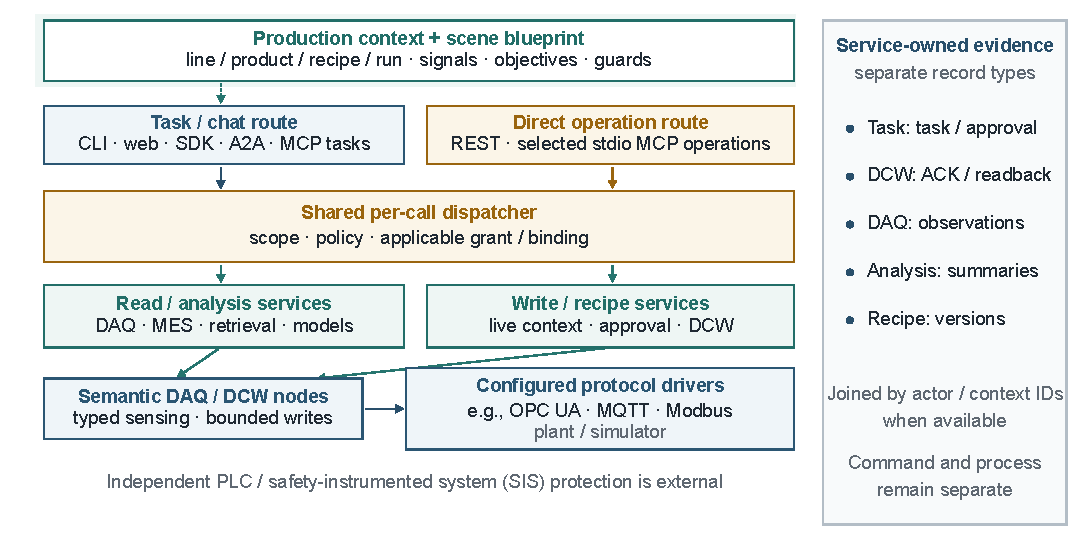
\includegraphics[width=\textwidth]{resources/fig-architecture-2026-9pt.pdf}
\caption{AgentWorkShop architecture and record ownership. Task/chat calls pass
through the listed access surfaces and a registered harness; direct REST and
selected stdio-MCP operation calls enter the shared dispatcher, while MCP
management/task methods use their service routes. R22 evaluates direct REST
operation calls; the stdio-MCP route is shown but not evaluated. Recipe writes recheck the
approved line--product--recipe--run tuple; each service retains its own
records. Independent programmable logic controller and safety-instrumented
system protection remains external.}
\label{fig:arch}
\end{figure*}
\section{System Design}
\label{sec:design}
AgentWorkShop is designed for industrial tasks whose agents, production
contexts, interfaces, and process signals vary between deployments. Its
architecture organizes these variations around shared task and operation
services, checks each proposed operation against the active production
context before device routing, and retains route-specific evidence that
distinguishes a command receipt from a measured process response.

\subsection{Design Rationale and Requirements}
\label{sec:principles}
Five requirements---scene variability, harness variability, operation
authority, outcome observability, and extensibility---organize six design
rules (D1--D6). These are deployment constraints drawn from the target
workflows. D1 stores scene settings as versioned data;
D2 provides registered harness, tool, and driver interfaces; D3 separates
proposal from execution; D4 treats the tool catalog as discovery rather than
permission; D5 routes actuator writes through the common DCW admission point;
and D6 retains evidence by operation.

The requirements trace to implementation as follows.
Scene variability maps to D1, scene blueprints, and context resolution;
harness variability and extensibility map to D2, the registered harness and
driver interfaces; operation authority maps to D3--D5, the shared dispatcher,
grants, bindings, and write admission; outcome observability maps to D6,
route-specific receipts, and observations. R20 and R21 exercise the
registered-harness path, while R22 exercises direct operation calls in two
scene-specific protocol mappings. Section~\ref{sec:eval} reports the
experimental scope and evidence limits. AgentWorkShop supplies task and
operation services; agent strategy and independent process protection remain
outside this design.

\subsection{Layered Architecture}
\label{sec:layers}
\label{sec:arch}
Fig.~\ref{fig:arch} summarizes the access routes, shared dispatch path,
production services, semantic I/O, configured drivers, and service ownership
of records. Task and chat routes enter the
collaboration band, which contains workspaces, channels, task queues, shared
memory, mailboxes, task templates, and harness adapters. Direct REST tool
calls and the stdio MCP operation bridge can call the shared dispatcher
without creating a task or invoking a harness; MCP management and task methods
remain on their service routes. Direct calls have no agent-turn prompt
context, so handlers resolve current route state from the request and services
at invocation. The governance band projects an operation catalog and
checks each invocation. The context band assembles bound-line and active-run
information for prompt grounding, while operation handlers resolve the live
state relevant to their route. The service band provides acquisition, write
control, analysis, retrieval, and optional model services. The field-I/O band
resolves semantic nodes to built-in or plugin drivers for a plant or
simulator.

Each band has a distinct responsibility. Task/chat routes enter the task
runtime; direct operation routes enter the dispatcher; and both use shared
operation checks where applicable. A harness adapter supplies
agent-specific interaction on task paths, semantic nodes hide protocol
details from operations, and the driver registry provides the device-facing
extension point. Owning services retain task, command, observation, and
version records separately and link them to available actor and production
context. No single status conflates these outcomes.

\subsection{Cross-Module Execution Flow}
\label{sec:executionflow}
Fig.~\ref{fig:runtime} summarizes a task turn from entry through operation
execution, with route-specific evidence retained by owning services. Registered
harness adapters receive a scoped tool catalog during setup and supported
registry refreshes; the runtime assembles prompt-time production context for
each agent turn. This context is grounding information, not a task-pinned
transaction. For each returned tool call, the shared dispatcher rechecks
invocation scope and channel policy and, for industrial operations, current
grant and binding conditions before handler selection. The selected handler
then applies route-specific guards, active-run checks, approval
revalidation, and device-I/O steps as applicable. Command receipts and later
process observations remain distinct records.

For an industrial operation $u$ by agent $a$ in channel $c$, define the
shared dispatch condition as
\begin{equation}
\mathcal{A}(a,c,u)=\bigwedge_{X\in\mathcal{C}(u)}X(a,c,u),
\label{eq:dispatch-contract}
\end{equation}
where $S$, $P$, $G$, and $B$ denote invocation scope, current channel policy,
runtime grant, and agent binding/resource ownership, respectively.
$\mathcal{C}(u)\subseteq\{S,P,G,B\}$ is the set of predicates declared for
operation $u$; it always contains $S$ and $P$. The grant predicate $G$ is
omitted only for an explicitly grant-exempt industrial tool, and $B$ is
included when the operation declares resource references. A declared
no-reference operation omits $B$. Each included check must pass before
handler selection. The policy predicate includes channel tool selection,
profile, and duty-separation checks where configured. This condition is
necessary for handler selection, not sufficient for actuation: the selected
route applies its own guards and approval, then rechecks authority, context,
and applicable limits before dispatch.

Fig.~\ref{fig:execution} gives reference pseudocode for the registered-harness
task path, not one literal orchestrator function. Direct REST tool invocation
bypasses the task runtime and harness but enters the same shared dispatcher.
Route-specific timing, approval, and evidence rules are detailed in
Section~\ref{sec:modules}.

\begin{figure*}[!t]
\centering
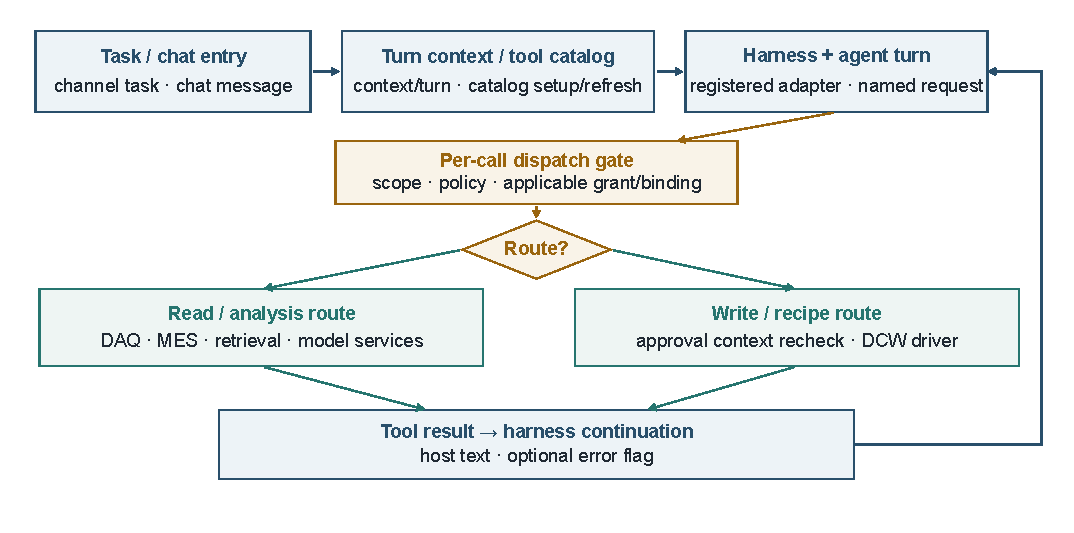
\includegraphics[width=\textwidth]{resources/fig-runtime-2026-9pt.pdf}
\caption{Registered-harness task flow. Context is assembled per turn; the
scoped tool catalog is loaded at setup or refresh. The dispatcher checks
scope, policy, and applicable grants and bindings, then returns each tool
result to the active harness turn. Direct REST and selected stdio-MCP
operations enter the shared dispatcher without a task. In R20, the follow-up
probe, ingest, and run-tagged query were initiated by the test runner outside
the agent task. A command receipt remains distinct from a process observation.}
\label{fig:runtime}
\end{figure*}

\begin{figure}[!t]
\centering
\begin{algorithmic}[1]
\Require task $q$, channel $c$, bound agent $a$, registered scoped catalog $T$
\Ensure task result; any retained evidence remains with its owning service
\State $x_t \gets \Call{ResolvePromptContext}{c,q}$
\State $m \gets \Call{RetrieveMemory}{q}$
\State $p \gets \Call{AssemblePrompt}{q,x_t,m}$
\State $h \gets \Call{InvokeRegisteredHarness}{a,p,T}$
\ForAll{tool request $u$ returned by $h$}
  \State $g \gets \Call{CheckScopeAndChannelPolicy}{a,c,u}$
  \If{\textbf{not} $g$}
    \State \Call{EmitToolErrorToHarness}{h,u}; \textbf{continue}
  \EndIf
  \If{$u$ is an industrial operation}
    \State $v \gets \Call{CheckGrantBindingOwnership}{a,u}$
    \If{\textbf{not} $v$}
      \State \Call{EmitToolErrorToHarness}{h,u}; \textbf{continue}
    \EndIf
  \EndIf
  \State $k \gets \Call{SelectHandler}{u}$
  \State $r \gets \Call{ExecuteRouteHandler}{k,a,c,u}$
  \Comment{handler resolves live state and may persist route-specific records}
  \State \Call{EmitDeclaredToolResultToHarness}{h,r}
\EndFor
\State \Return task state and tool results
\end{algorithmic}
\caption{Reference pseudocode for the registered-harness task path.
Direct operation invocation is not shown. Evidence persistence is
route-specific and remains with the owning service; the shared tool result
does not carry a generic evidence envelope.}
\label{fig:execution}
\end{figure}

\section{Module Functions and Integration}
\label{sec:modules}
The architecture in Fig.~\ref{fig:arch} is implemented as cooperating
modules rather than a single monolithic agent. Shared interfaces connect
task execution to configuration, industrial services, protocol drivers, and
route-specific evidence. This section describes those responsibilities and
the checks that preserve their boundaries.

The implementation scope is broader than the evaluated scope. Section~V
separates implemented interfaces from the routes and checks exercised here;
an interface intended for extension does not by itself establish
interchangeability or portability.

The extension contracts expose the data passed at each boundary. A harness
call is normalized as \texttt{HostToolCall(toolName, arguments)} and returns
\texttt{HostToolResult(text, isError)}. A DCW driver accepts an engineering
value, tolerance, range, and driver configuration; its result separates write
status, raw value, readback, and acknowledgment grade (readback-verified,
transport-ack, or unverified). Each DAQ sample stores its node, timestamp,
value, and state, with optional line, product, recipe, and run IDs. A write
anchor records line/node, prior and requested values, source, actor, time, and
optional run/task/approval IDs; recipe definitions retain separate versions.
These fields keep tool errors, device receipts, observations, and production
lineage inspectable as separate records.

DAQ and write-anchor records may omit line, product, recipe, run, task, or
approval identifiers when a route does not supply them. For the R20 trace
audit, the join keys are required: task ID, approval ID, recipe-trial run ID,
active-run ID, and the run ID returned with the sample must agree with the
corresponding route records. R21 checks the corresponding IDs on its
deterministic fixture path. Thus the reported complete joins are requirements
of those evaluated records, not a guarantee that every general record
contains every identifier.

\subsection{Task Runtime and Harness Adapters}
Task and chat access surfaces create or join a workspace channel, where the
task engine manages members, task queues, shared memory, and execution
templates. Direct REST tool calls and selected stdio MCP operation calls can
enter the shared dispatcher without creating a task or invoking a harness;
MCP management and task methods use their corresponding services. A direct
call has no agent-turn prompt context: its operation handler resolves live
route state from request identifiers and service data at invocation.
The harness registry instantiates an adapter behind a common agent interface;
the prompt builder combines the task with the active scene brief, industrial
context, channel profile, agent binding, and retrieved memory. Tool calls
return to the shared dispatcher regardless of which registered harness
produced them. The registry keeps engine-specific execution behind the common
agent interface. Industrial context is assembled for
each agent turn rather than pinned for the task lifetime, so prompt context is
grounding information rather than write authorization. An approved recipe
action separately captures the current line--product--recipe--run tuple when
approval is requested and compares it again before dispatch. This
approval-time check does not imply that the earlier prompt context remained
unchanged.

\subsection{Production Context and Configuration}
Scene blueprints describe devices, signal maps, objectives, and process
guards. A task resolves these definitions against its active
line--product--recipe--run context. The channel profile selects the available
capability family, the tool policy narrows the operation catalog, and the
agent binding scopes the nodes, controls, and recipe operations available to
that member. These filters can restrict one another but cannot broaden the
underlying device range. The dispatcher re-reads policy at execution, so a
cached catalog does not retain authority after a grant or policy change. The
prompt builder assembles the agent's available bound-line and active-run
context on each turn; it does not pin the complete context tuple to the task.
Approved recipe actions capture the active tuple at request time and refuse
dispatch if its line, product, recipe, or run field changes during the
approval wait.
Specific production snapshot, trial, and MPC routes, together with Hybrid Twin
training submissions, resolve and validate a versioned \texttt{SceneContract}
at operation time. The Twin physics-specification draft route can instead
accept a caller-supplied scene description; SceneContract enforcement is
therefore route-specific and does not validate or pin all prompt context.

\subsection{Acquisition, Analysis, and Modeling Services}
Semantic DAQ nodes expose typed values, engineering units, ranges, and
sampling settings while hiding protocol-specific reads. A per-node DAQ
runtime schedules acquisition and stores timestamped observations; the
gateway aggregates node pipelines. MES-facing operations provide the
configured production-data path. Analysis and retrieval services consume
these records, while optional model, training, optimization, and digital-twin
services are invoked through their registered operation handlers. These
services complement the agent workflow; AgentWorkShop does not prescribe a
single optimization strategy.

\subsection{Semantic I/O and Actuation}
The driver registry resolves a semantic node to a built-in or plugin driver.
DAQ handlers use the node's acquisition interface; DCW handlers route a
write or readback through the controller and the configured protocol driver.
This separation lets recipes and agents refer to semantic controls without
embedding Modbus, OPC UA, MQTT, HTTP, or MES transport details in their
operation arguments. The supported driver mappings are implementation
interfaces; only the mappings and workflows enumerated in Section~\ref{sec:eval}
are experimentally exercised.

\subsection{Shared Dispatch and Write Admission}
\label{sec:governed}
Every named operation passes the dispatcher. Its ordered checks validate
invocation scope and current channel policy (tool selection, profile, and
applicable duty separation), then the agent's binding and runtime grant and
ownership of referenced resources.
A refusal returns the excluding condition. Denial persistence is selective:
grant denials and selected resource-reference denials have explicit audit
paths, whereas scope and channel-policy denials are not uniformly retained as
durable audit events. A catalog entry therefore describes availability but
does not authorize execution. Handlers for operations that require manual
approval suspend for a decision, then revalidate authority and active limits
before dispatch. For manual recipe operations, the handler checks the active
run, candidate parameters, and route timing before approval; after the wait it
rechecks current authority and active limits. For \texttt{recipe\_apply}, a
changed definition requires a new proposal. These route-specific checks
complement, but do not replace, the per-call dispatcher checks.

All actuator writes converge on the DCW admission point. For an online node
write, the admissible interval is
\begin{equation}
\mathcal{I}^{\mathrm{online}}_n(t)=\mathcal{H}_n\cap\mathcal{B}_n
\cap\mathcal{P}_n(t)\cap\mathcal{R}_n(t),
\label{eq:admission}
\end{equation}
where $\mathcal{H}_n$ is the hard engineering range and $\mathcal{B}_n$,
$\mathcal{P}_n$, and $\mathcal{R}_n$ are the baseline, active-product, and
active-recipe limits. Missing optional limits impose no restriction, whereas
an empty intersection rejects the request and identifies the excluding
layer. Recipe dispatch applies the hard, baseline, and product limits to the
replacement recipe rather than intersecting with the previous recipe window.
The actuator path also enforces step, interval, and hold-window checks.
These admission rules constrain commands; process objectives and coupled
variable guards are assessed from later observations. The framework does
not replace independent PLC or safety-instrumented protection.

\subsection{Integrated Operation and Route-Specific Evidence}
\label{sec:tasklifecycle}
A recipe trial illustrates how the modules cooperate. The task runtime
delivers a named \texttt{recipe\_trial} call from the agent harness; the
dispatcher checks the agent's recipe binding and execution scope; the recipe
handler checks the active run, candidate parameters, and route timing; and a
manual binding requests approval before the DCW controller sends the batch
through its driver. The handler returns a per-parameter receipt. The caller
then obtains DAQ observations and can request a separate update, apply, or
rollback operation. A trial receipt confirms command handling; it does not
by itself establish process attainment or persist a new recipe version.

The routes retain different records because they answer different
questions. A driver acknowledgment reports command evidence; DAQ reports a
process observation; an exploration summary records a bounded probe; and a
recipe version records a saved definition. Their relation through actor and
production context allows an execution to be inspected without treating
these outcomes as interchangeable.

\subsection{Route-Specific Lifecycles and Evidence}
\label{sec:routes}
\label{sec:mech}
\label{sec:objective}
\label{sec:nodeexec}
\label{sec:ack}

\paragraph{Timing and approval}
Timing guards are route-specific. Online node writes enforce an effective
minimum spacing of 60\,s. Recipe dispatch uses a per-recipe interval anchored
to approval, while trials also use a configurable per-line cadence (default
300\,s). The recipe interval can refuse a proposal before an approval request
is created. Checks occur at proposal or execution according to the operation,
and experiment-specific pacing overrides are reported with the corresponding
results.

Manual bindings create an approval request containing the actor, operation,
candidate values, applicable limits, expiry, parameter bases, and the active
line--product--recipe--run context. The default wait expires after 180\,s and
refuses execution. After approval, the executor rechecks authorization and
compares the current context tuple with the approved tuple. For approved
recipe writes and dispatched rollback, a final synchronous comparison follows
the asynchronous grant check immediately before entering the DCW dispatch
path. Changes visible at this software boundary are refused before a driver
write. This check is not an atomic lock across network or device I/O and
cannot cancel a driver call after it begins. A focused mock-state suite
changes line, product, recipe, or run during approval for recipe apply, trial,
and dispatching rollback; each mutation is refused before a driver write or
new execution record. For
\texttt{recipe\_apply}, a changed recipe definition also requires a new
proposal; an unchanged approval dispatches a copy of the approved parameter
snapshot. A line-level recipe mode defaults to manual; changing it to
automatic requires administrator confirmation. The approval record
authorizes a workflow action and does not replace process protection.

Fig.~\ref{fig:hitl}(a) illustrates the four-layer interval in
Eq.~(\ref{eq:admission}) with an archived RPM configuration; panel (b) shows a
symbolic approval followed by context and authority rechecks. The plotted
values are illustrative and are not R20 measurements.

\begin{figure*}[!t]
\centering
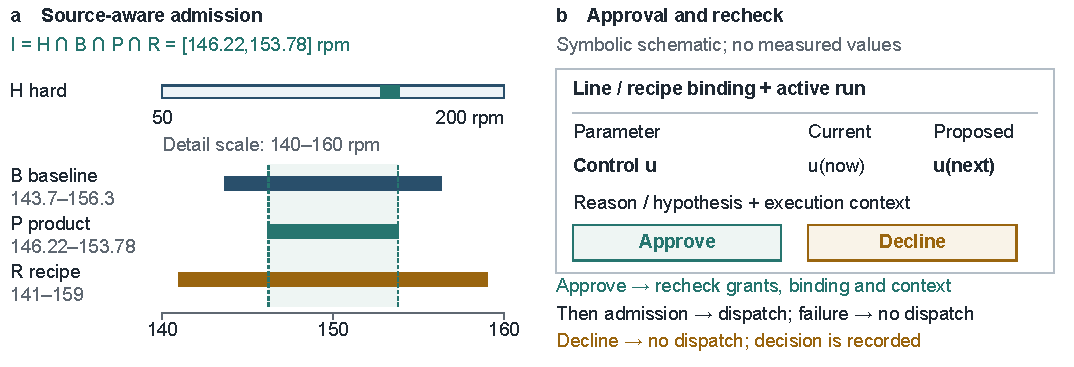
\includegraphics[width=\textwidth]{resources/fig-admission-hitl-2026.pdf}
\caption{Admission and approval boundaries. (a) Illustrative archived RPM
configuration (not part of R20):
online node interventions use the four-layer value interval of
Eq.~(\ref{eq:admission}),
whereas recipe dispatch omits the prior recipe window. (b) Symbolic human
approval binds a proposed action and its context tuple; execution rechecks the
active line--product--recipe--run context, authority, and applicable limits
after approval. Approval does not reserve equipment state.}
\label{fig:hitl}
\end{figure*}

\paragraph{Node probe}
The bounded \texttt{optimization\_explore} route is exposed to the AML
optimization profile. It validates a bound control and DAQ scope, captures a
baseline, routes a bounded write through DCW, and stores a later target window
as a separate exploration summary. Its timing and approval behavior is
route-specific; R20 does not exercise this route.

\paragraph{Recipe operations}
\texttt{recipe\_trial} checks the bound recipe and active run, then dispatches
candidate overrides as a batch with per-parameter verification. The caller
subsequently queries DAQ and may save a definition with
\texttt{recipe\_update}, restore one with \texttt{recipe\_rollback}, or apply
a version with \texttt{recipe\_apply}. A trial does not save or apply a
version, and endpoint verification is not a process-response measurement.
Public direct-node control is closed; bounded probes and recipe operations are
the configured write surfaces.

\paragraph{Command verification}
Command confirmation and process response answer different questions. A
driver ACK is graded as \texttt{readback-verified}, \texttt{transport-ack},
or \texttt{unverified}; a matching endpoint read supports the first grade,
whereas transport or MES application confirmation supports the second.
Recipe-batch verification is \texttt{verified}, \texttt{unverified}, or
\texttt{failed}. If readback is absent or mismatched, up to three reads are
attempted 2\,s apart. Initial ACKs, final ACKs, and per-parameter verdicts are
retained separately. A readback-verified setpoint does not establish target
attainment.

\paragraph{Observation, verdict, and compensation}
Recipe-path observation follows batch dispatch, and saving a definition,
applying it, and observing process response remain separate operations. An
open node record can request rollback after repeated breaches; missing samples
do not count as breaches. Caller verdicts and compensation remain separate
from the observation and subject to admission checks.
\label{sec:agentloop}


\FloatBarrier
\section{Experimental Evaluation}
\label{sec:eval}
The evaluation asks whether registered-harness tasks and direct operation calls
can execute bounded recipe actions across two simulator scenes with different
signal and protocol mappings while retaining route-appropriate records. R20 is
the primary result: six sequential tasks through one registered harness, three
per scene on one simulator instance per scene, with task-to-approval-to-receipt-
to-sample links. R21 is a deterministic fixture replay of the registered-
harness path; R22 separately exercises the direct operation endpoint without a
task or harness. All runs use repository simulators. Supplementary File~S1
contains their separate records, scripts, and trace checks.

\subsection{Evidence Units and Experimental Procedure}
\label{sec:testbed}
\label{sec:procedure}
R20 uses the registered harness adapter named \texttt{omp} in cast-film and
annealing scenes
(\texttt{omp} is the project adapter key, not a network protocol),
with three sequential task executions per scene on one simulator instance per
scene. Each execution creates a new logical line, product, recipe, active run,
channel, agent, and task on that shared scene simulator. Line start reapplies the recipe baseline
(120~rpm or 730~$^{\circ}$C), so the control read returns to baseline while
the simulated process state carries forward. These are sequential software
runs, not independent process replications. R21 and R22 use fresh isolated
application/simulator environments and are reported separately from R20.

Table~\ref{tab:routes} summarizes the evaluated paths and their inference
limits; Table~\ref{tab:q8} gives the six R20 process snapshots.

\begin{table*}[!t]
\centering
\caption{Evaluation paths, recorded outcomes, and inference limits. The route
counts are kept separate because the runs use different entry paths and
execution modes.}
\label{tab:routes}
\footnotesize
\setlength{\tabcolsep}{3pt}
\begin{tabularx}{\textwidth}{@{}p{1.25cm}p{3.4cm}X p{4.0cm}@{}}
\toprule
Path & Execution & Recorded outcome & Inference limit \\
\midrule
R20 & Six sequential tasks through one registered harness; three per scene. & 6/6 task--approval--receipt--sample links; six verified receipts; all six single probes were outside target. & One simulator per scene; one probe per task; no process-attainment claim. \\
R21 & One deterministic fixture task per scene on the registered-harness route. & 2/2 fixture traces; 31 runner assertions passed. & No external model decision or independent process replication. \\
R22 & One direct operation call per scene, without a task, harness, or language-model decision. & 2/2 calls approved; each returned a 1/1 verified receipt and matching readback, then one active-run-tagged snapshot; both were outside target; 19 checks passed. & No task-to-sample link; one snapshot per scene; no alternate-harness portability claim. \\
Context tests & Twelve stale-context mutations on three recipe routes; production handler and test-only ablation. & Production handler refused 12/12 before writes; one queued post-recheck change was also refused. Without tuple equality, six product/run mutations triggered 12 mock writes and six execution records. & Temporary/mock state; component ablation, not a platform baseline or physical safety test. \\
\bottomrule
\end{tabularx}
\end{table*}

\subsection{Registered-Harness Process Path (R20)}
\label{sec:harness-e2e}
R20 ran the local v0.8.0 working-tree application with the registered
\texttt{omp} adapter and GLM-5.3-Flash. Supplementary File~S1 lists the source
reconstruction requirements; credentials are omitted and external model
decisions are not deterministic. Cast-film used OPC UA control and MQTT
thickness sensing; annealing used Modbus TCP for control and sensing. In each
scene the model selected one value from a prevalidated candidate set for a
bounded \texttt{recipe\_trial}, and a synthetic administrator approved it.
Each route record contains one 1/1 readback-verified receipt. After verifying
the receipt, the runner waited 20~s, probed and ingested one sample, and queried
it by active-run ID through the isolated SQLite fallback. All six tasks
completed and passed 76 runner assertions. The trace audit found 6/6 complete
task--approval--receipt--sample links. The trial-operation run ID differs from
the active production-run ID used for the sample; both link through the task
and approval. Task state was checked after sampling, so completion-to-sample
latency is unavailable. Table~\ref{tab:q8} reports all six values and
identifiers are in the S1 trace matrix. All samples remained outside target;
one probe per task does not measure process response or normal online DAQ.

\begin{table}[!t]
\centering
\caption{Bounded recipe-trial settings and post-readback simulator probes. All
six samples remained outside their target bands.}
\label{tab:q8}
\footnotesize
\setlength{\tabcolsep}{2.5pt}
\begin{tabularx}{\columnwidth}{@{}lXcX@{}}
\toprule
Case & Pre-task value / target band & Control: start$\to$trial & Sample \\
\midrule
Film-1 & $55.82/48$--$52~\mu$m & $120\to125$~rpm & $45.69~\mu$m \\
Film-2 & $45.69/48$--$52~\mu$m & $120\to130$~rpm & $46.69~\mu$m \\
Film-3 & $46.69/48$--$52~\mu$m & $120\to125$~rpm & $45.69~\mu$m \\
Anneal-1 & $675.40/700$--$760~^{\circ}$C & $730\to745$~$^{\circ}$C & $679.60~^{\circ}$C \\
Anneal-2 & $678.30/700$--$760~^{\circ}$C & $730\to745$~$^{\circ}$C & $677.70~^{\circ}$C \\
Anneal-3 & $676.90/700$--$760~^{\circ}$C & $730\to745$~$^{\circ}$C & $678.10~^{\circ}$C \\
\bottomrule
\end{tabularx}
\end{table}

\subsection{Deterministic Fixture Replay (R21)}
R21 used a deterministic transport fixture for the registered \texttt{omp}
adapter, without an LLM decision. One task per scene exercised approval,
verified receipt/readback, and a run-tagged sample; all 31 runner checks,
including cleanup, passed. This is a replay of the same harness route, not an
independent agent or process replication, and is reported separately from R20.

\subsection{Direct Operation Endpoint (R22)}
R22 used a fresh isolated environment. A worker identity issued one direct
\texttt{recipe\_trial} call per scene through
\texttt{/api/workshop/agent-tools/invoke}, without a task, harness transport,
or external model. Synthetic approval produced a 1/1 verified receipt and
matching readback for each call. After 20~s, one sample per scene was queried
by active-run ID: 46.37~$\mu$m versus a 48--52~$\mu$m band and 675.20~$^{\circ}$C
versus a 700--760~$^{\circ}$C band. All 19 checks passed. This tests a direct
entry route and two mappings, not process response or cross-harness
portability; R22 is separate from R20 and R21.

\subsection{Software Contract Checks}
The local unit suite passed 566/566 tests across seven suites. In the 20-case
approval suite, twelve injected line, product, recipe, or run changes across
three recipe routes were refused before mock writes or new execution records.
One queued post-recheck context change was also refused before dispatch. In a
test-only ablation that removed tuple equality but retained authority and
limit checks, six product/run changes caused twelve mock writes and six
execution records; independent checks still blocked line/recipe changes.
This component ablation shows the tuple check's incremental software-state
coverage, not a platform baseline or safety guarantee. Tests use mock or
temporary state and do not establish atomicity during device I/O or test
end-to-end DAQ tag failures.

\section{Discussion}
\label{sec:limits}
R20 produced six complete task-to-approval-to-receipt-to-sample traces across
two simulator scenes; none of its single post-readback samples reached target.
R21 passed 31 assertions on the deterministic registered-harness route. R22
separately exercised two direct operation calls, one per simulator scene;
both returned verified receipts and run-tagged snapshots, with each snapshot
outside its target band. A 20-case mock suite refused twelve stale
approval-context mutations across three recipe actuation routes before
actuation. A test-only ablation that removed tuple-equality checks allowed the
product and active-run mutations to proceed on all three routes, while
independent checks still blocked line and recipe changes. This isolates the
added coverage of the tuple check for those two context fields; it is a
component ablation, not a baseline comparison with another integration
framework. A separate queued-context test confirms refusal before the handler
resumes dispatch after the asynchronous grant check.

Each scene used one simulator instance and a single post-readback probe per
task; the results therefore do not establish independent process replication,
convergence, or quality improvement. R22 covers direct operation entry but
does not test another registered harness. Configuration reuse, normal online
data acquisition, physical transfer, and comparative architecture value
remain untested. The context comparison is a software-state check at the
dispatch boundary, not a lock across asynchronous device I/O or external
process transitions. Synthetic approval does not measure
operator effectiveness
\cite{parasuramanmanzey2010complacency,parasuraman2000model,bainbridge1983ironies};
tool restrictions do not establish deployment security
\cite{greshake2023injection,liu2024pinjection,iec62443-3-3} or replace
independently engineered PLC/SIS protection \cite{iec61511}. Future work
should compare a defined platform-level baseline and include independent
simulator and physical-plant trials.

The positive-path records evaluated here do not constitute a complete durable
denial ledger. In particular, scope and channel-policy refusals are not
uniformly persisted, so auditability claims are limited to the route records
and denial classes explicitly described in Section~IV.

\section{Conclusion}
\label{sec:conclusion}
AgentWorkShop connects collaborative tasks and direct operation calls to
production context, checked operations, semantic I/O, and service-owned
records. R20 and R21 verify selected registered-harness paths, and R22
verifies a direct operation endpoint across two simulator mappings. Mock-state
tests confirm refusal when the approved context changes before dispatch; the
ablation isolates added refusal coverage for product and active-run changes.
These results validate selected software behavior, not platform-level
comparative integration value or process performance.


% Identity-neutral acknowledgment: documents AI assistance without exposing authors.
\section*{Acknowledgment}
OpenAI ChatGPT revised Sections~I--VI and drafted Python for Figs.~1, 2, and
4. OpenAI image generation produced early concepts for Figs.~1 and 2; final
vectors were redrawn and implementation-checked. AI generated no experimental
records or measurements. The authors verified all submitted content.

\bibliographystyle{IEEEtran}
% Keep IEEEtran's default bibliography size and leading.
\bibliography{resources/refs}

\end{document}
